\chapter{Evaluation}
\label{chapter:evaluation}

metrics: accuracy / F1 / AUR, number of genes, processing time

LOOCV vs 10-fold CV

\section{Benchmarking Setup}
\label{sec:benchmarkSetup}

For the experiments, data from The Cancer Genome Atlas (TCGA) was downloaded from the Genomic Data Commons (GDC) using the TCGAbiolinks package\cite{colaprico2015tcgabiolinks,grossman2016toward,weinstein2013cancer}. 
We selected 8 different cancer types because of their good coverage in DisGeNET (GBM, HNSC, KIRC, LAML, LUAD, SARC, THCA, UCEC). 
We filtered out all genes and samples that had more than 30\% missing values. 
Afterwards, the data was normalized by library size and log-transformed using the VST\cite{durbin2002variance} procedure. 
After preprocessing, the dataset consisted of 3,189 samples and expression values for 55,572 genes. 

\section{Experiments}
\label{sec:experiments}

First, we ran computational and the DisGeNET based FS on this dataset. 
We selected our computational FS approaches according to recommendations from Bol\'{o}n-Canedo et al.\cite{bolon2014review,bolon2013review}.
They conclude that IG, ReliefF and SVM-RFE are the best approaches in their respective categories of univariate filter, multivariate filter and embedded.
We did not use any wrapper approach because of their high complexity and no clear advantages over filter or embedded methods.
Additionally, we used a variance-based FS (VB-FS) because it is very fast and used a lot to filter genes in differential gene expression workflows.

Next, we produced combinations of the feature rankings from VB-FS and IG with the unranked gene sets from the knowledge bases DisGeNET and KEGG.
The combination with VB-FS and IG was chosen because they are simple methods that are able to quickly rank features. 

All of those feature rankings were evaluated on the dataset using 10-fold cross validation with the classifiers SVM, Logistic Regression, Naive Bayes and KNN (with k=3;5) by averaging their classification accuracy.

%kannst du hier vielleicht noch ein zweites oder drittes datenset mal durch dein evaluation-framework durchlaufen lassen (um zu zeigen, dass diese ergebnisse nicht spezifisch für dieses datenset sind)?
%accuracy % averaged over 10-fold CV classification with SVM, Logistic Regression, Naive Bayes and KNN with K=3;5

Fig. \ref{fig:accuracy} compares DisGeNET based FS, computational methods and combined approaches. 
All computational methods outperform DisGeNET with 4+ genes used. 
From the computational methods, IG performs best up until 6 genes selected while after that SVM-RFE achieves the best performance.

\begin{figure}[h!]
\setlength{\belowcaptionskip}{-15pt}
\centering
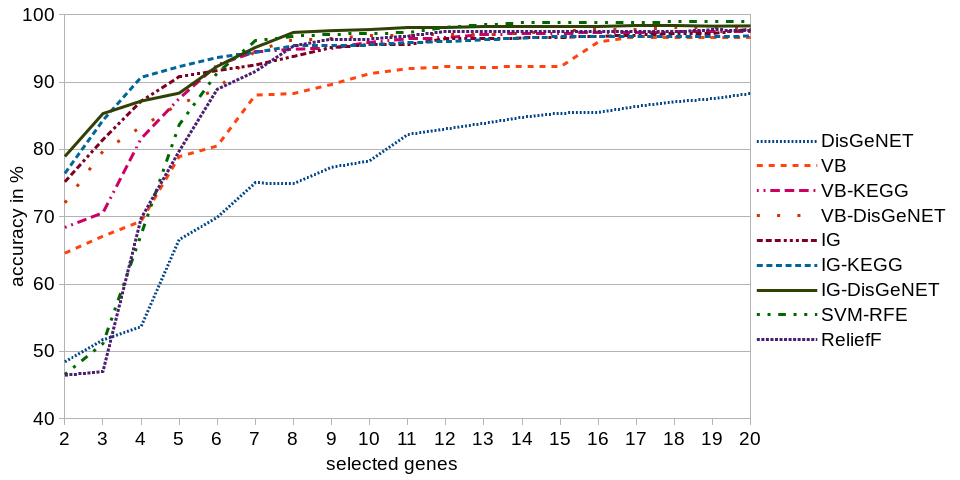
\includegraphics[width=0.95\textwidth]{figures/accuracy5.png}
\caption{Combination feature ranking by using knowledge base extracted genes as a filter for the computational feature ranking}
\label{fig:accuracy}
\end{figure}

Moreover, all combination approaches perform better than the DisGeNET method alone. 
The VB-FS combinations perform similarly and both improve over using only VB-FS. 
The same holds true for the IG combinations which perform best overall up until 12 genes.
After that SVM-RFE performs best.
At 17+ genes, all approaches apart from DisGeNET plateau and perform similarly with accuracies between 96\% and 98\%. 

\section{Discussion}
\label{sec:discussion}

As the results show, knowledge based FS gets outperformed by computational methods. 
However, enriching simple methods like VB-FS and IG with prior knowledge improves performance.
Every combination is able to compete with complex methods like SVM-RFE.  
Another advantage of the combined approach is its low complexity and thus low execution time.
This makes it useful for large datasets.
The biological interpretability of the chosen genes by using prior knowledge and simple statistical methods is another advantage.

There are some limitations to the proposed combined approach though. 
We require knowledge of which diseases are contained in the dataset to map them to the knowledge bases for the automatic selection of biologically relevant genes.
In addition, sufficient information about those diseases needs to exist in the knowledge bases.
However, as biological knowledge bases gather more data through research on diseases like cancer and Alzheimer, our approach will become more viable and useful in an increasing number of scenarios in the future.

In order to further verify our results, the combined FS method integrating prior knowledge should be tested with other datasets and other diseases. 
A more in-depth study with more computational methods and integrating more prior knowledge could show even better results for combinations or reveal cases where the integration of biological knowledge is especially useful. 
The developed framework enables and encourages this because of its flexibility which allows for the integration of diverse datasets, FS methods and external knowledge sources.
